\chapter{Results \& Discussion}
\label{Chapter4}
\lhead{Chapter 4. \emph{Results \& Discussion}}

\section{Convergency Tests}
\subsection{Cut-off Energy}
\subsection{K-Points Sampling}
\section{Density of States (DOS)}



Hello
\begin{figure}[H]
    \centering
    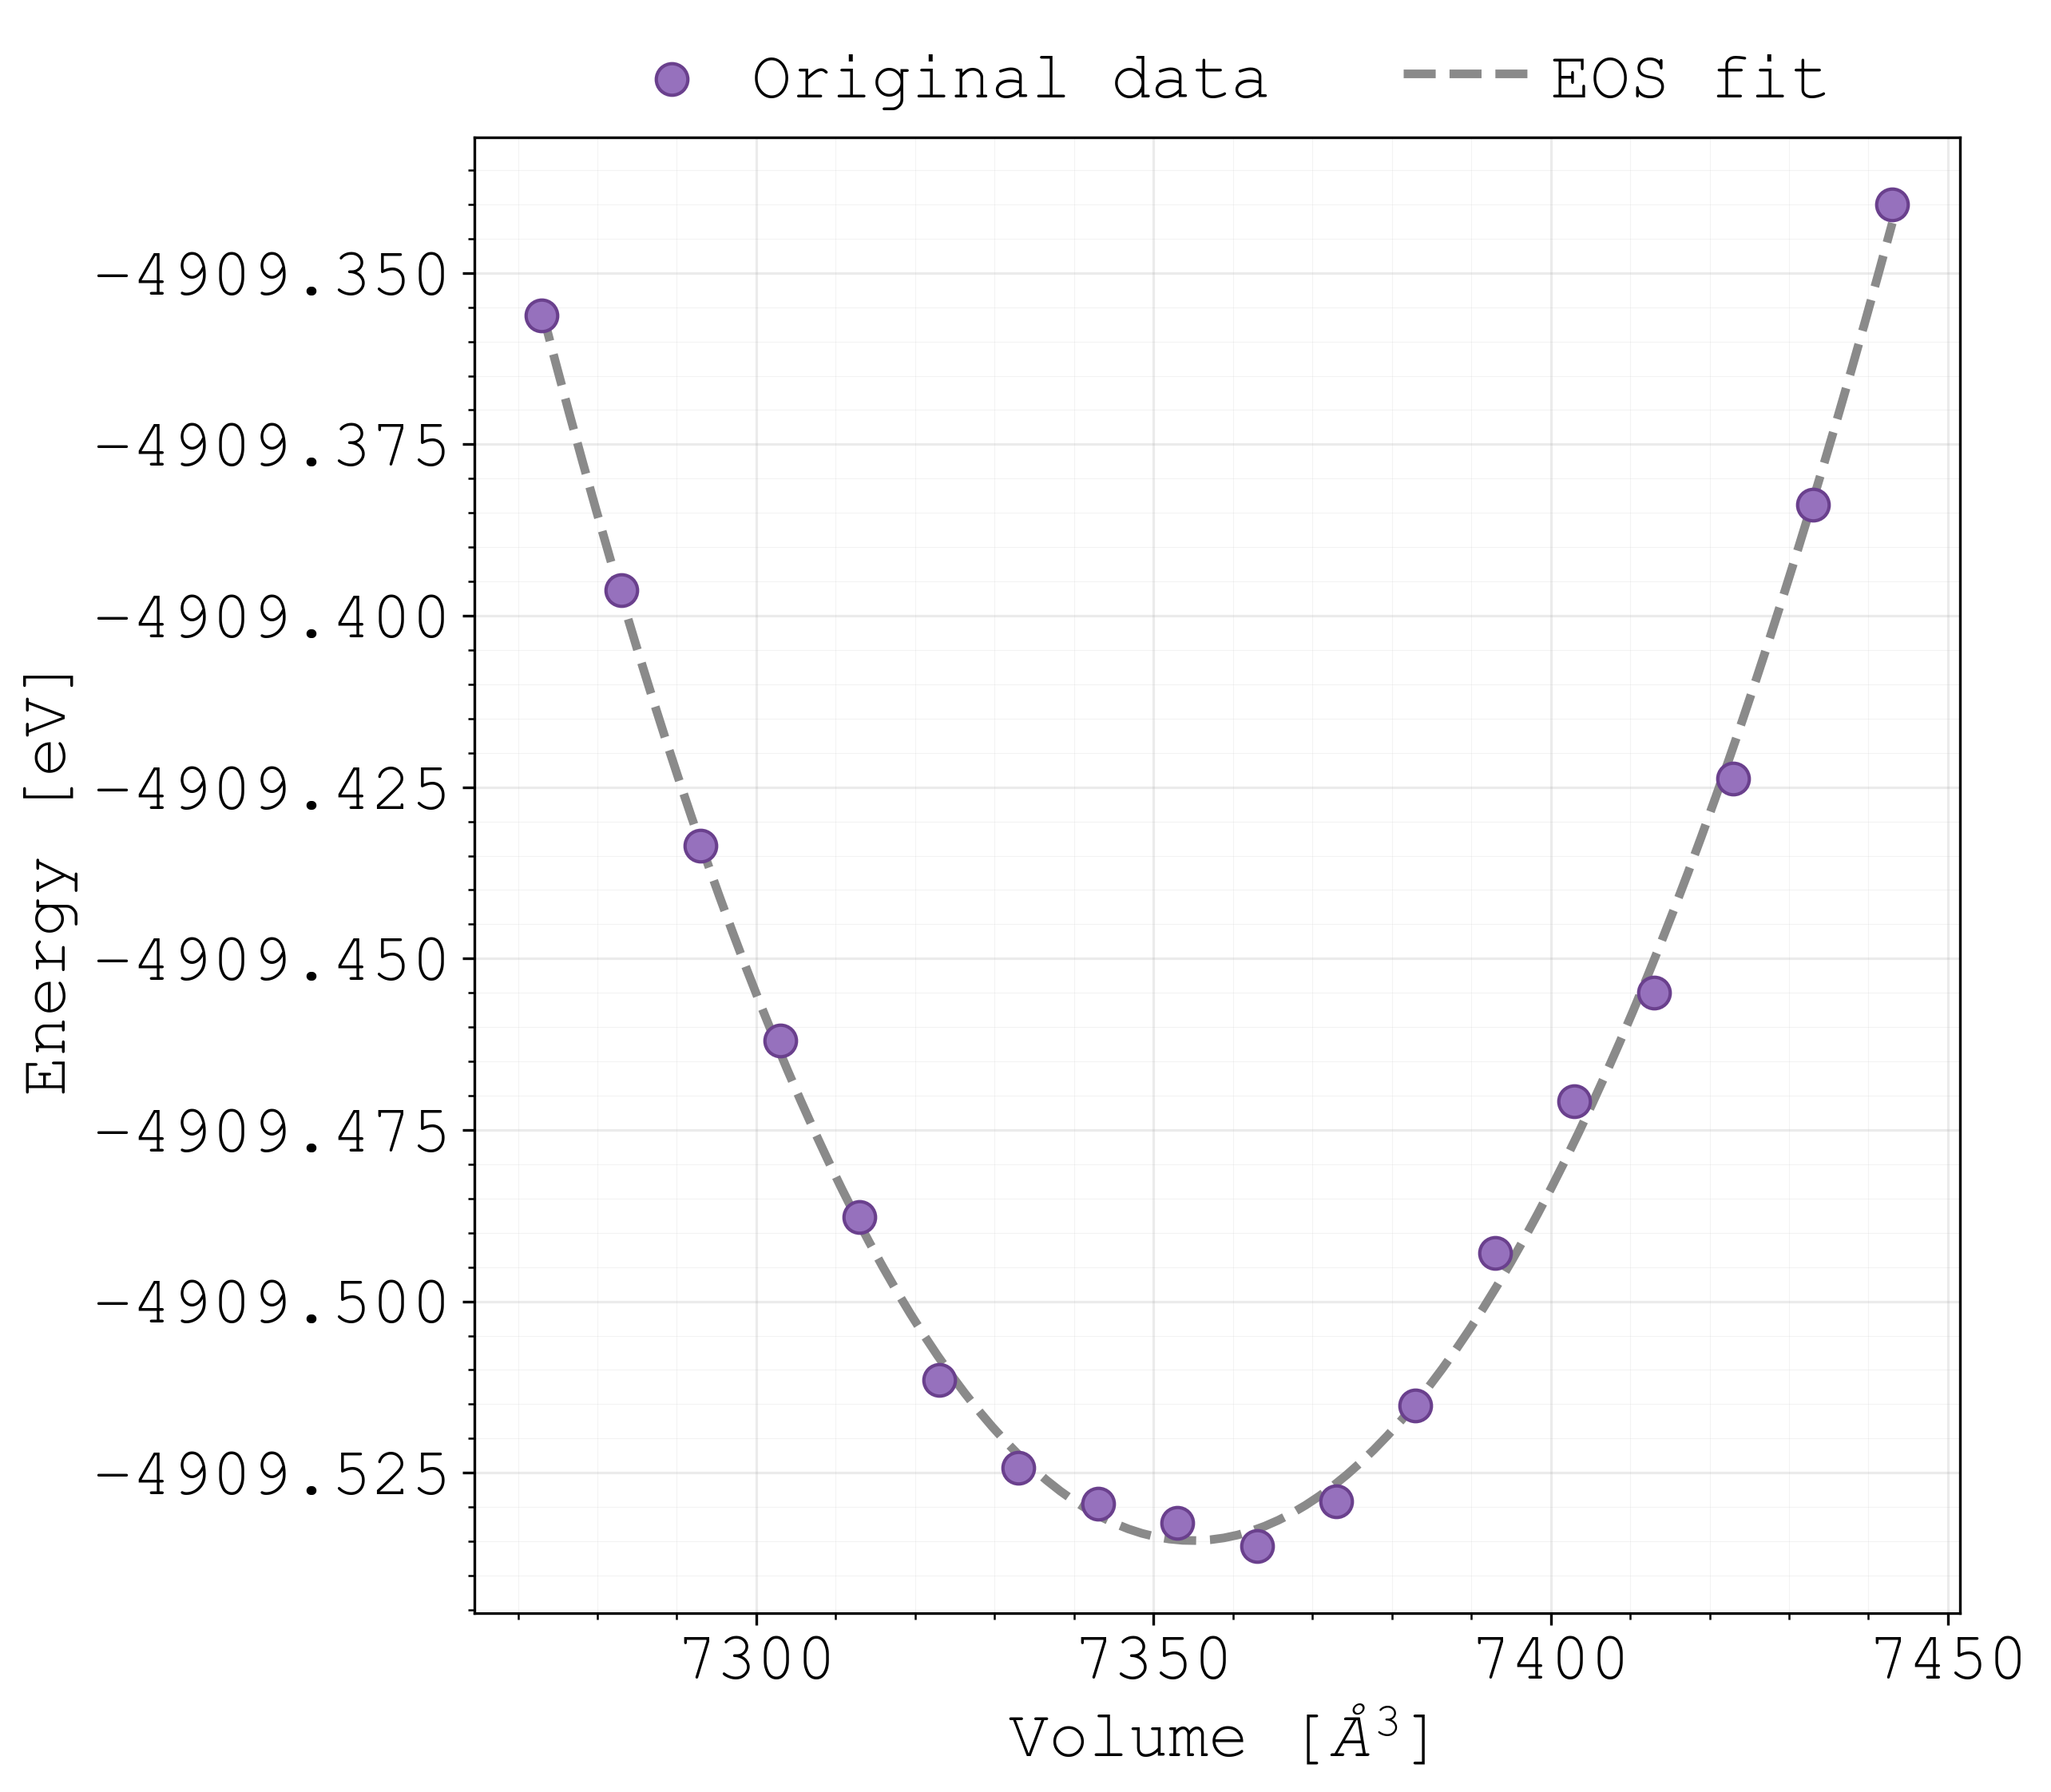
\includegraphics[width=0.7\textwidth]{EOS_SA_EDIFF_02.png}
    \caption{A schematic representation of the DFT formalism. The many-body wavefunction is replaced by a single-particle wavefunction, which is used to calculate the electron density. The electron density is then used to calculate the total energy of the system. Adapted from \supercite{giustino2014materials}.}
    \label{fig:dft}
\end{figure}
